\documentclass[problem]{mcs}

\newcommand{\neutr}{\ensuremath{\mathbf{N}}}

\begin{pcomments}
  \pcomment{CP_3color_OR_gate}
  \pcomment{forked and shortened from PS_3color_SAT}
  \pcomment{ARM Fall '11, edited by CH Spring '14}
\end{pcomments}

\pkeywords{
SAT
logical_formula
propositional_logic
logic
proposition
negation
coloring
}

%%%%%%%%%%%%%%%%%%%%%%%%%%%%%%%%%%%%%%%%%%%%%%%%%%%%%%%%%%%%%%%%%%%%%
% Problem starts here
%%%%%%%%%%%%%%%%%%%%%%%%%%%%%%%%%%%%%%%%%%%%%%%%%%%%%%%%%%%%%%%%%%%%%
\begin{problem}

In this problem, we examine an interesting connection between
propositional logic and 3-colorings of certain special graphs.  In the
graph shown in Figure~\ref{fig:3color-OR}, designate the vertices
connected in the triangle on the left as \emph{color-vertices}.  Since
each color-vertex is adjacent to the other two, they must have
different colors in any coloring of the graph.  The colors assigned to
the color-vertices will be called $\true, \false$ and $\neutr$.  The
dotted lines indicate edges to the color-vertex $\neutr$.

\begin{figure}%\inbook{[h]}
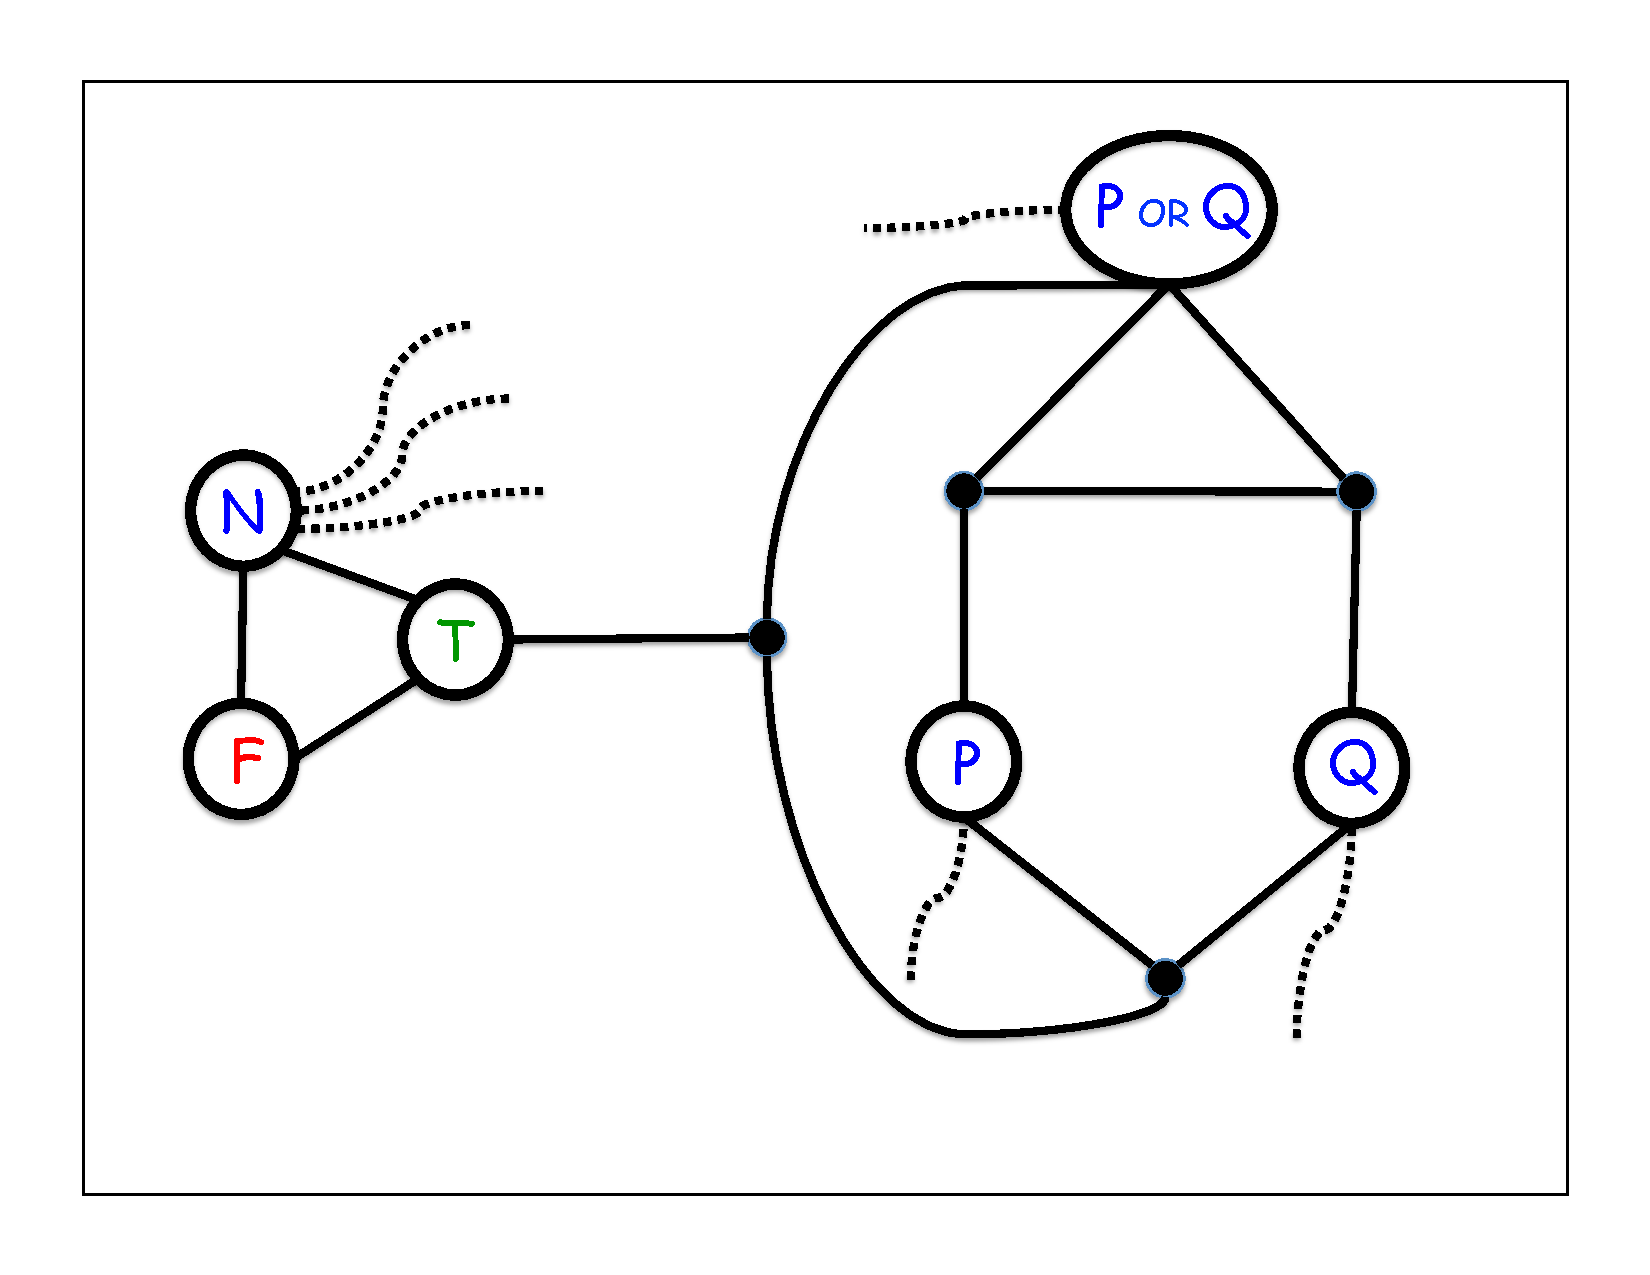
\includegraphics[width=4in]{3color-OR}
\caption{A 3-color $\QOR$-gate}
\label{fig:3color-OR}
\end{figure}

\bparts

\ppart Prove that there exists a 3-coloring of the graph iff neither $P$
nor $Q$ are colored $N$.

\begin{solution}

%\begin{proof}

\textbf{(left-to-right case)}: If there is a valid 3-coloring (or more
generally, any valid coloring) then the dotted edges ensure that $P$
and $Q$ are not colored as $\neutr$ in that coloring.

\textbf{(right-to-left case)}: If neither $P$ nor $Q$ are colored $\neutr$,
then both $P$ and $Q$ have to be colored $\true$ or $\false$.  

The diagram is symmetric in $P$ and $Q$, so there are really only
three cases to consider: $P$ and $Q$ are both colored $\true$, both
colored $\false$, or $P$ and $Q$ are colored differently.  If $P$ and
$Q$ are colored differently, we can verify that this leads to only one
possible 3-coloring where the vertex labelled $(P \QOR Q)$ is colored
$\true$.

If $P$ and $Q$ have the same color, then one of the vertices directly
above must be colored with $\neutr$ and the other with the opposite color
as $P$ and $Q$.  This forces $(P \QOR Q)$ to be colored
with the same color as $P$ and $Q$.  There is then a unique coloring
of the bottom vertex, and the middle vertex on the arc on the left that
can complete a 3-coloring.

Therefore, in each case where neither $P$ nor $Q$ are colored $\neutr$,
there exists a valid 3-coloring.

%\end{proof}

\end{solution}

\ppart Argue that the graph in Figure~\ref{fig:3color-OR} acts like a
two-input $\QOR$-gate: a valid 3-coloring of the graph has the vertex
labelled $(P \QOR Q)$ colored $\true$ iff at least one of the vertices
labelled $P$ and $Q$ are colored $\true$.

\iffalse
\hint Examine the relation between the colors of $P$, $Q$ and $(P \QOR
Q)$ in your solution to the first part. 
\fi

\begin{solution}
We can think of $P$ and $Q$ as ``input'' vertices and $(P \QOR Q)$ as
the ``output'' vertex.  In the argument above, we concluded that when
$P$ and $Q$ have different colors, $(P \QOR Q)$ is colored
$\true$.  On the other hand, when $P$ and $Q$ have the same color, then $(P
\QOR Q)$ also shares this color.  Therefore, the color of $P
\QOR Q$ is always the Boolean $\QOR$ of the colors assigned to $P$ and
$Q$. 

\end{solution}

\ppart Changing the endpoint of one edge in Figure~\ref{fig:3color-OR}
will turn it into a two-input $\QAND$ simulator.  Explain.

\begin{solution}
Change the endpoint of the horizontal edge incident to the
$\true$-vertex to be incident to the $\false$ vertex.

As before, when $P$ and $Q$ have the same color, the ``$(P \QOR
Q)$''-vertex must to be colored with the same color.  Likewise, if $P$
and $Q$ are colored differently, then the bottommost vertex must be
colored $\neutr$ which forces the leftmost black vertex, which is now
incident to the $\false$ vertex, to be colored $\true$, forcing the
``$(P \QOR Q)$''-vertex to be colored $\false$.

Hence, with this edge change, the ``$(P \QOR Q)$''-vertex is now
really a $(P \QAND Q)$-vertex.
\end{solution}
\eparts

\end{problem}

%%%%%%%%%%%%%%%%%%%%%%%%%%%%%%%%%%%%%%%%%%%%%%%%%%%%%%%%%%%%%%%%%%%%%
% Problem ends here
%%%%%%%%%%%%%%%%%%%%%%%%%%%%%%%%%%%%%%%%%%%%%%%%%%%%%%%%%%%%%%%%%%%%%

\endinput
